\section{Calibration accuracy and residual non-Gibbs distortion}
\label{sec:calibration}

This section reports what is already measurable with exact enumeration at small $N$: how far a calibrated annealer sample actually sits from the intended visible distribution, independent of any $\betaeff$ fit.

\subsection{Effect of input scale and automatic normalization}

Figure~\ref{fig:autoscale} sweeps the input coefficient scale $\beta_x$ on a small ($N=8$) Pegasus-embedded network. With the solver's automatic coefficient normalization enabled, rescaling all programmed coefficients by $1/\beta_x$ has little effect on either $\DTV(\widehat q,\pi_\theta)$ or the fitted $\widehat\beta_{\mathrm{LS}}$: normalization divides by a quantity that scales with the same factor, canceling the intended change. With normalization disabled, both quantities respond to $\beta_x$: the recorded $\DTV$ falls from $\approx0.63$ to $\approx0.30$ near $\beta_x=5$ before rising again, against a finite-sample reference of $\approx0.19$ at this sample count. Reaching the right scale improves the histogram; it does not make the sampled distribution statistically indistinguishable from an ideal sample of $\pi_\theta$ at that sample count.

\begin{figure}[t]
\centering
\panel{.48}{\textbf{(a)}\\
\includegraphics[width=\linewidth]{figures/dtv_autoscale_dtv_N8.pdf}}\hfill
\panel{.48}{\textbf{(b)}\\
\includegraphics[width=\linewidth]{figures/dtv_autoscale_beta_N8.pdf}}
\caption{Effect of automatic coefficient normalization on a small ($N=8$) Pegasus-embedded network. (a) Total-variation distance to the enumerated $\pi_\theta$. (b) Fitted $\widehat\beta_{\mathrm{LS}}$ (Eq.~\eqref{eq:cem-ls}). Disabling normalization lets the input scale $\beta_x$ change the sampled law; enabling it cancels the attempted adjustment. The reference line is a finite-sample floor at this sample count, not a lower bound.}
\label{fig:autoscale}
\end{figure}

\subsection{Sampler comparison against the exact trial distribution}

Figure~\ref{fig:classical} compares classical samplers against the exactly enumerated distribution of trained $N=M=8$ networks at two field values. Metropolis and block Gibbs sampling remain close to the finite-sample reference across the tested effort range; simulated annealing starts far from it at low effort and approaches the other two as its schedule lengthens. A separate audit of the source report (\texttt{audyt\_cld\_bg.md}, finding O2: ``No matched QPU-versus-classical sampling-quality benchmark'') asked for exactly this comparison on a QPU. We obtained one directly: 10 fresh Pegasus draws (200 reads each, live \texttt{Advantage\_system6}, $\beta_x=2.0$) on a small trained network ($N=8$, from the surviving \texttt{cem\_validation} checkpoint), scored against the same exact-enumeration reference used throughout this section -- $\DTV(\widehat q,\pi_\theta)=0.637$ (IQR $[0.620,0.641]$) and $\widehat\beta_{\mathrm{LS}}=1.80$ (IQR $[1.66,1.85]$) across the 10 seeds. This sits well above the classical samplers' finite-sample floor in Fig.~\ref{fig:classical} -- a real, live-hardware instance of the residual non-Gibbs distortion this section is built around, not merely the single differently-scoped auto-scale point of Fig.~\ref{fig:autoscale}.

\begin{figure}[t]
\centering

\includegraphics[width=\linewidth]{figures/dtv_classical_N8_M8.pdf}\\[2pt]
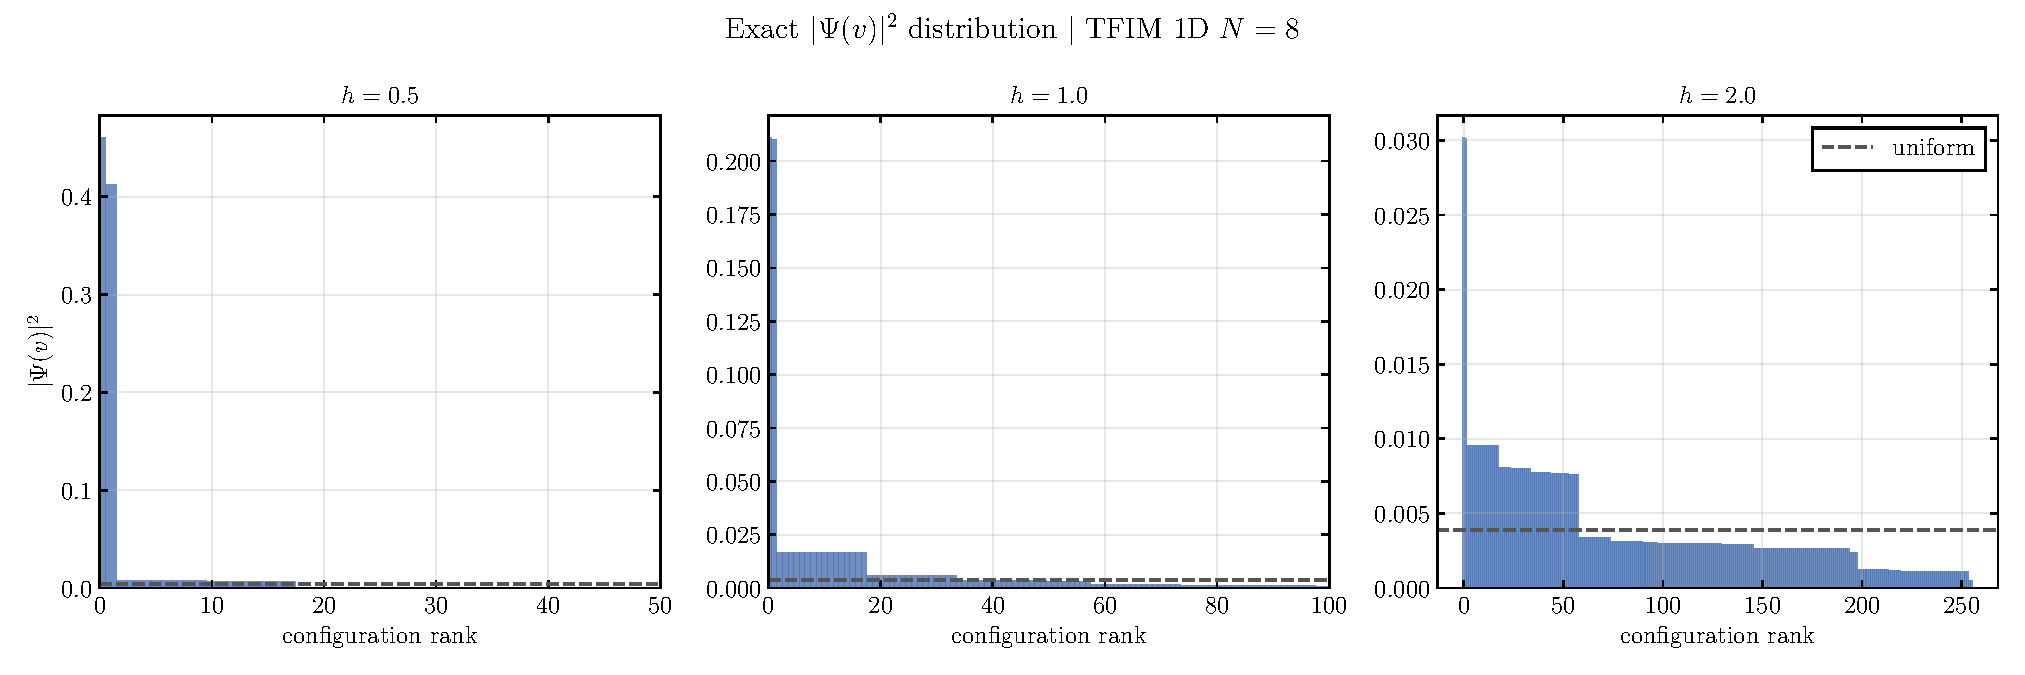
\includegraphics[width=\linewidth]{figures/dtv_classical_N8_M8_dist.pdf}
\caption{Sampling diagnostics for trained $N=M=8$ Ising networks at $h=0.5$ and $h=2$. Top: total-variation distance from the enumerated trial distribution vs.\ sampling effort. Bottom: ranked probabilities of the trial distribution itself.}
\label{fig:classical}
\end{figure}

A matched comparison turns out to already exist in the archived training logs, just never plotted this way. Every training run at $N\le16$ logs \texttt{kl\_exact}: the exact-enumeration $\DKL(\widehat q\Vert\pi_\theta)$ between that iteration's empirical sample histogram and the \emph{current} $\theta$'s own exactly enumerated Born distribution (\texttt{src/encoder.py}, gated by \texttt{KL\_EXACT\_MAX\_N=16}), computed identically for classical and QPU-driven runs. Figure~\ref{fig:kl-solver} plots it against SR iteration for all six solvers at $N=8,16$, closing audit finding O2 above with no new experiments.

\paragraph{Status.} \textbf{O2: closed}, in substance: a matched classical-vs-QPU sampling-quality comparison, on identical axes, now exists at $N=8,16$. One narrower part of the original finding is not fully addressed -- it also asked for the fitted $\beta_{\mathrm{eff}}$ to be reported alongside; we show CEM's downstream effect on distributional fidelity (Fig.~\ref{fig:kl-cem}) rather than tabulating $\widehat\beta_{\mathrm{LS}}$ itself next to Fig.~\ref{fig:kl-solver}.

\begin{figure*}[t]
\centering
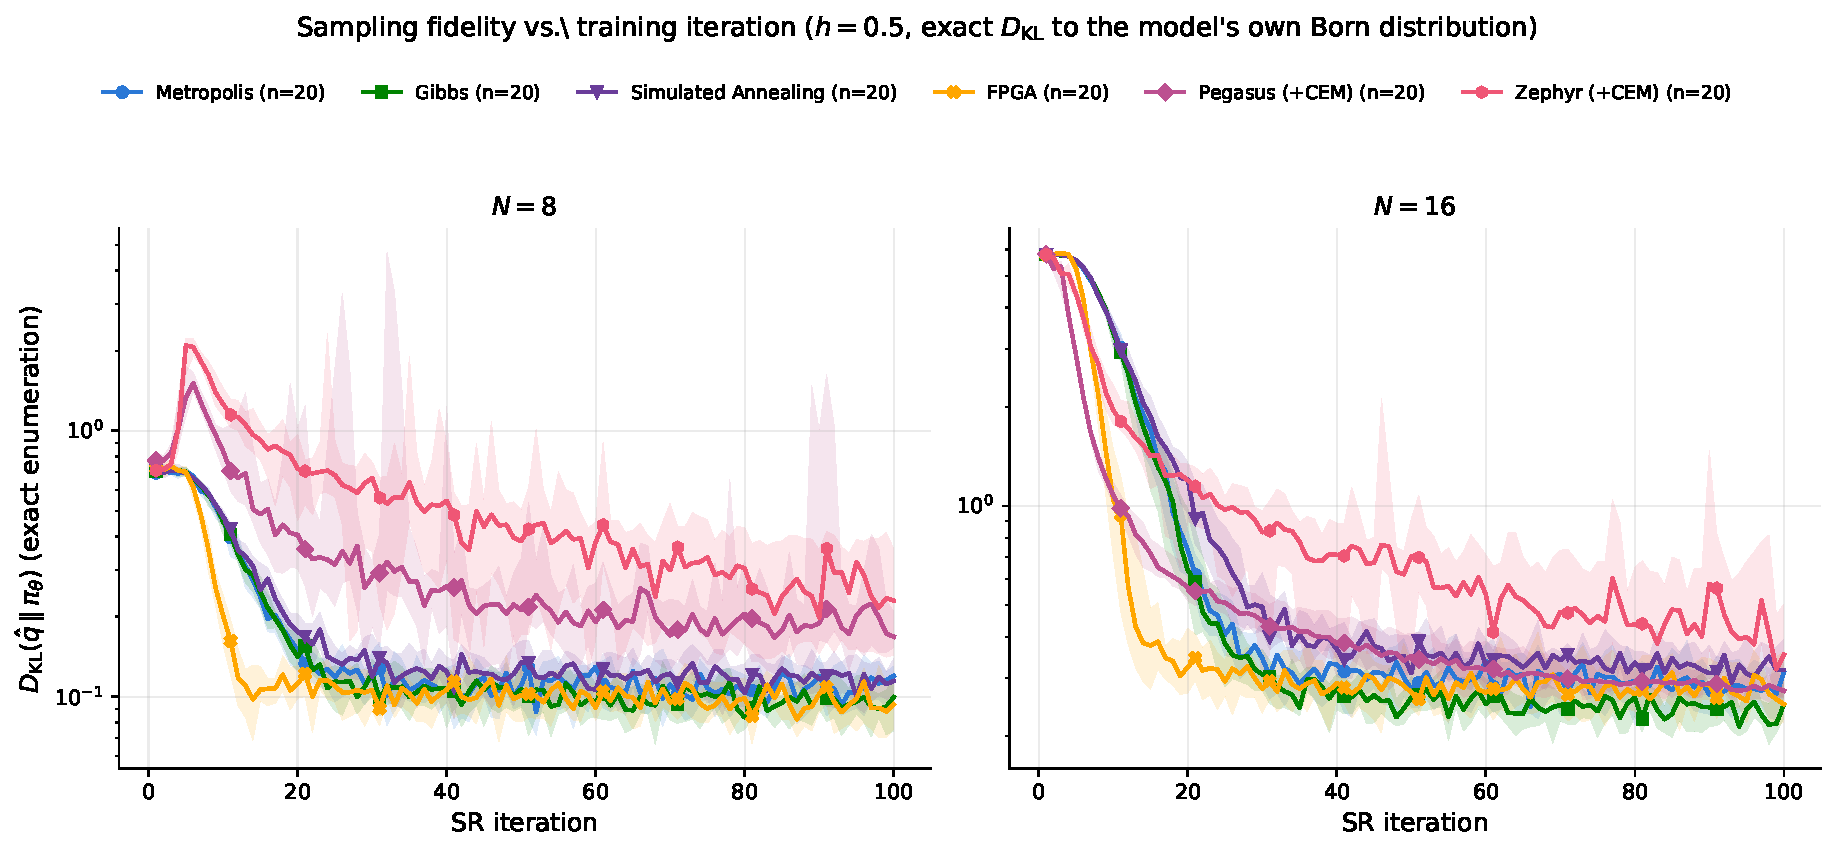
\includegraphics[width=\textwidth]{figures/reanalysis/fig_kl_exact_solver_comparison.pdf}
\caption{Exact $\DKL(\widehat q\Vert\pi_\theta)$ vs.\ SR iteration, $h=0.5$, $N=8,16$ (median and IQR band, 20 seeds per solver). Classical MCMC (Metropolis, Gibbs, simulated annealing) and FPGA converge to a common, tight floor by iteration $\sim\!20$--$30$. Pegasus(+CEM) and Zephyr(+CEM) settle above that floor, with visibly wider bands -- a directly quantified, exact-enumeration version of the ``residual non-Gibbs distortion'' this section otherwise only measures indirectly through $\DTV$ at one instance. All curves start high and decline: the RBM's own Born distribution is close to unstructured at initialization, and concentrates onto a lower-entropy manifold as SR training proceeds, which is mechanically easier for a finite sample to resolve regardless of sampler -- confirmed by Metropolis, whose $\beta_x$ is fixed at exactly $1$ throughout and shows the same decline. Pegasus(+CEM) and Zephyr(+CEM) additionally show an early rise before falling; we checked and ruled out a simple explanation (their $\beta_x$ is already fluctuating in its eventual steady range during this rise, not still converging from a poorly calibrated start), so the mechanism behind the hump is left as an open question rather than asserted.}
\label{fig:kl-solver}
\end{figure*}

The same data lets us test the paper's own central claim directly: does pooled CEM correction actually improve distributional fidelity, or only training-energy stability? Figure~\ref{fig:kl-cem} compares \texttt{cem=0} against \texttt{cem=1} for both devices. CEM lowers the median final-iteration $\DKL$ by a factor of $\approx\!4$ for Pegasus ($0.66\to0.17$ at $N=8$; $1.26\to0.27$ at $N=16$) and $\approx\!10$ for Zephyr ($2.57\to0.23$ at $N=8$; $3.72\to0.35$ at $N=16$), durably across the entire training run rather than only at convergence.

\begin{figure*}[t]
\centering
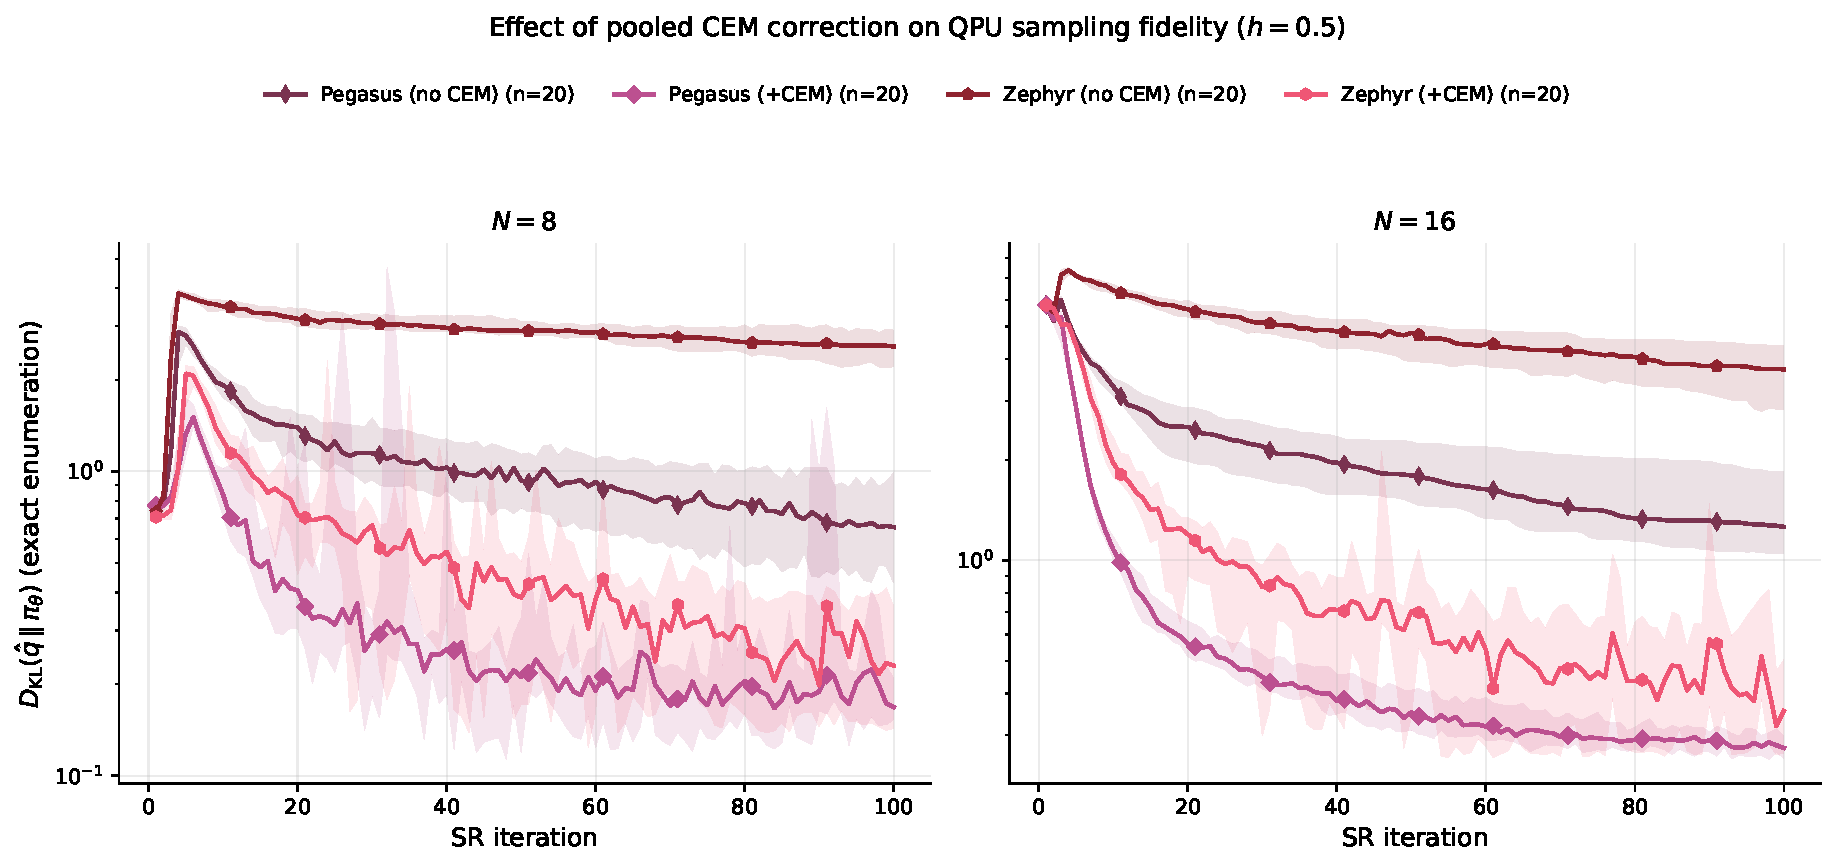
\includegraphics[width=\textwidth]{figures/reanalysis/fig_kl_exact_cem_ablation.pdf}
\caption{Effect of pooled CEM correction on exact $\DKL(\widehat q\Vert\pi_\theta)$, $h=0.5$, $N=8,16$ (median and IQR band, 20 seeds per arm). \texttt{cem=0} (uncorrected) sits nearly an order of magnitude above \texttt{cem=1} throughout training for both devices, with the larger benefit for Zephyr. This is direct evidence that the pooled-CEM estimator of Sec.~\ref{sec:cem-ls} improves the sampled distribution itself, not only the logged training energy.}
\label{fig:kl-cem}
\end{figure*}

Both figures are scoped to $N\le16$ by the same \texttt{KL\_EXACT\_MAX\_N} enumeration limit discussed in Sec.~\ref{sec:validation}; they say nothing directly about $N=64$, where the crossover of Sec.~\ref{sec:limitations} is reported.

\subsection{Consistency between conditional and visible fits}

Figure~\ref{fig:cemvalidation} compares the pooled-CEM estimate $\widehat\beta_{\mathrm{LS}}$ against a direct visible-distribution fit $\widehat\beta_{\mathrm{KL}}=\arg\min_\beta\DKL(\widehat q\Vert\pi_{\theta,\beta})$, obtainable only where $\pi_{\theta,\beta}$ can be enumerated ($N=8,12$). Many points lie near the diagonal, but checkpoint-averaged offsets of order $0.06$–$0.08$ appear, and at least one fit sits at the search boundary $\beta=50$. Agreement is therefore neither uniform nor evidence of exact calibration; it is consistent with -- but does not by itself demonstrate -- the counterexample of Sec.~\ref{sec:cem-limits}, in which the pooled hidden loss can be minimized at the correct $\beta$ even when the visible marginal is substantially wrong.

\begin{figure}[t]
\centering
\panel{.48}{\textbf{(a)}\\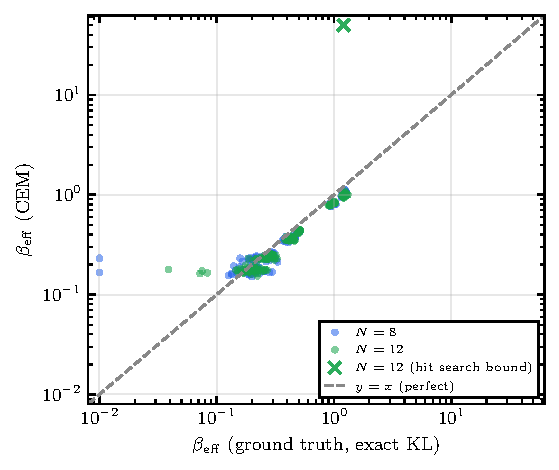
\includegraphics[width=\linewidth]{figures/cem_validation_calibration.pdf}}\hfill
\panel{.48}{\textbf{(b)}\\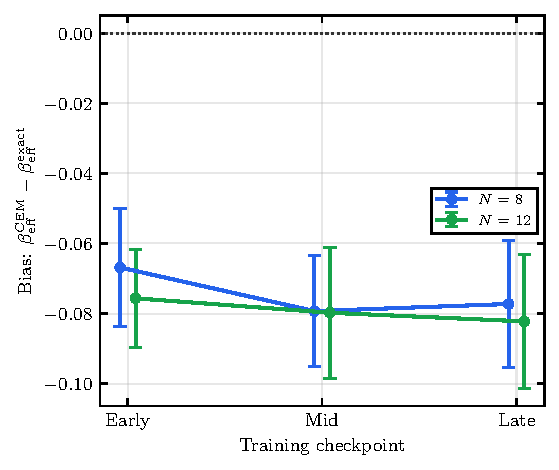
\includegraphics[width=\linewidth]{figures/cem_validation_bias.pdf}}
\caption{(a) Pooled-CEM $\widehat\beta_{\mathrm{LS}}$ against the enumerated visible-fit $\widehat\beta_{\mathrm{KL}}$, $N=8,12$. (b) Checkpoint-averaged offsets. A boundary estimate is annotated and must not be read as a resolved optimum.}
\label{fig:cemvalidation}
\end{figure}

Figure~\ref{fig:cem} illustrates the least-squares fit itself for a representative $N=16$ network: the pooled conditional loss $\mathcal L(\beta)$ has a clear minimum distinguishing $\widehat\beta_{\mathrm{LS}}\approx1.94$ from the candidates $\beta\in\{0.5,1,5\}$.

\begin{figure}[t]
\centering
\panel{.48}{\textbf{(a)}\\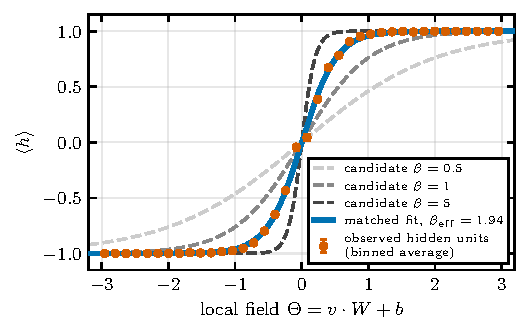
\includegraphics[width=\linewidth]{figures/cem_matching_candidates.pdf}}\hfill
\panel{.48}{\textbf{(b)}\\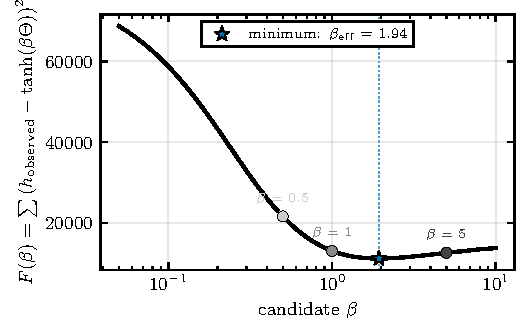
\includegraphics[width=\linewidth]{figures/cem_matching_objective.pdf}}
\caption{Pooled least-squares CEM for a representative $N=16$, $h=1$ network. (a) Binned hidden responses against candidate conditional curves. (b) $\mathcal L(\beta)$, Eq.~\eqref{eq:cem-ls}, minimized near $\beta=1.94$.}
\label{fig:cem}
\end{figure}

\missing{\textbf{Residual reported as a number, not only ``very close.''} Per the evaluation, Fig.~\ref{fig:cemvalidation} and Fig.~\ref{fig:cem} should be accompanied by numerical RMSE, relative error, bias, and boundary-hit frequency across the full $(N,h,\beta_x,\mathrm{seed})$ grid, not a qualitative description. This is a re-tabulation of already-collected fit results and does not require new hardware time, but no script currently outputs these summary statistics (Sec.~\ref{sec:code-gaps}).}

